\documentclass[10pt,a4paper]{article}
\usepackage[utf8]{inputenc}
\usepackage[russian]{babel}
\usepackage[OT1]{fontenc}
\usepackage{amsmath}
\usepackage{amsfonts}
\usepackage{amssymb}
\usepackage{graphicx}
\usepackage{authblk}
\usepackage{tabularx,ragged2e,booktabs,caption}
%\author{Столяров В.А.}


\begin{document}

\title{Проект радиоинтерферометра РИФ-32}  

\date{\today}

\author[1,2,3]{Столяров В.А.\thanks{vlad@sao.ru}}
\author[2,3]{Мингалиев М.Г.}
\author[2]{Сотникова Ю.В.}
\affil[1]{Cavendish Laboratory, University of Cambridge, UK}
\affil[2]{Специальная Астрофизическая Обсерватория РАН}
\affil[3]{Казанский Федеральный Университет}

\renewcommand\Authand{ и }
\renewcommand\Authands{ и }

	\maketitle
	\abstract{
В статье рассматривается проект системы апертурного синтеза для радиоастрономических наблюдений РИФ--32 ({\bf{Р}}адио{\bf{И}}нтер{\bf{Ф}}ерометра — 32). Инструмент из 32-х антенн планируется установить на территории САО РАН, где уже существует необходимая инфраструктура и есть кадровый потенциал для реализации такого проекта. Ядро радиоинтерферометра будет находится на территории РАТАН-600 и прилегающих участках, с длиной базы до 2.5 км. Отдельные антенны будут вынесены на ВНП (длина базы до 24 км). Также возможна установка одной антенны на территории радиоастрономической обсерватории «Зеленчукская» (длина базы 5 км). 
}


\section{Введение}
В настоящее время в России не существует радиоинтерферометра с компактным заполнением (u,v) плоскости. Единственный радиоинтерферометр «Квазар»  состоит из трёх инструментов, разнесённых на несколько тысяч километров (Приозерск, Зеленчукская, Бадары), которые включены в сеть VLBI.
В мире существует небольшое число инструментов предлагаемого типа, таких как VLA (США), ASKAP (Австралия), MeerKAT (ЮАР), а также более мелких, таких как AMI (Великобритания), получение наблюдательного времени на которых для российских астрономов затруднено. MeerKAT и ASKAP, которые являются наиболее близкими аналогами предлагаемого инструмента, расположены в Южном полушарии, как и проектируемый радиоинтерферометр SKA. В Северном полушарии единственным аналогичным инструментом является VLA. Расположенный в Европе LOFAR работает на более низких частотах, и не может заменить собой предлагаемый интерферометр, хотя и даёт в перспективе возможность проведения совместных наблюдений в широком частотном диапазоне.

Список задач, который можно решать на инструменте этого класса, довольно обширен. Сюда входят исследования эпохи реионизации, пульсарные исследования, наблюдения нашей Галактики, сознание каталога далёких объектов на космологических красных смещениях.

Предлагаемый инструмент будет единственным в России, где возможно решение всех этих задач.

В случае быстрой реализации проекта ввод инструмента в эксплуатацию возможен в 2023-2025 гг. Как показывает практика, время жизни радиоастрономических инструментов такого класса составляет порядка 50 лет. Предполагается, что инструмент SKA, где будут использованы аналогичные антенны производителя CETC54 (Китай), будет работать 50-60 лет после завершения строительства.

\section{Актуальность проблемы}

\section{Описание инструмента}

\subsection{ Технические характеристики}

\begin{minipage}{\linewidth}
\bigskip
\centering
\captionof{table}{Технические характеристики РИФ--32} \label{tab:rif32} 
\begin{tabular}{l|l}
  \hline
  Тип инструмента & радиоинтерферометр \\
  Количество антенн & 32 \\
  Тип антенны & Схема Грегори,\\ 
  & первичное зеркало 18х15 метров,\\ 
  & вторичное зеркало 5 х 4.7 метров \\
  Диапазон частот & 0.35 — 15.0 ГГц \\
  Чувствительность, $A_{eff}/T_{sys}$ & 200-220 $m^2/K$ \\
  Ширина полосы анализа &	До 1 ГГц \\
  Количество спектральных каналов & До 32768 \\
  Тип приёмников & криогенный \\
  Длина базы & 0.1 – 25 км \\
  Максимальное разрешение & 0.165 угл. сек.\\
  \hline
\end{tabular}
\bigskip
\end{minipage}

\subsection{Размещение и конфигурация РИФ--32}

\subsubsection{Размещение антенн}

Наиболее оптимальное место для размещения антенн с точки зрения логистики, коммуникаций и охраны – участок к югу от РАТАН-600, вытянутый вдоль трассы Р265. Его длина составляет порядка 2.5 км, ширина от 500 м до 1 км.
Предполагается, что отдельные антенны будут вынесены на ВНП (длина базы до 23 км).
Также возможна установка одной антенны на территории радиоастрономической обсерватории «Зеленчукская» (длина базы 5 км, Рис.~\ref{fig:RIF32-location}).

\begin{figure}
\center{
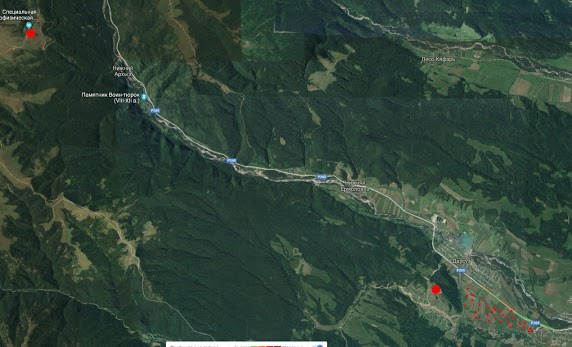
\includegraphics[width=1\linewidth]{./figures/RIF32-location}
%\includepdf[width=1.36\linewidth, page=1]{./figures/Correlator64_scheme}
}
\caption{Размещение антенн в "длинной" конфигурации. Основная группа антенн располагается вблизи РАТАН-600, одна антенна на территории р/а "Зеленчукская" (базы до 5 км), вторая - на ВНП (базы до 23 км). Антенны обозначены красными метками.}
\label{fig:RIF32-location}
\end{figure}

\subsubsection{Регулярная конфигурация}
Антенны располагаются по прямым линиям в виде рукавов (лучей) из центра инструмента (Рис.~\ref{fig:RIF32-config}a). В случае РАТАН-600 данный вариант неоптимален, т.к. из-за геометрии площадки доминирует компонента, расположеная по направлению Север-Юг, что неоптимально с точки зрения апертурного синтеза и приводит к существенным артефактам при работе алгоритма CLEAN.

\subsubsection{Случайная конфигурация}
Антенны располагаются по результатам моделирования Монте-Карло, с оптимизацией баз по равномерности заполнения uv-плоскости (Рис.~\ref{fig:RIF32-config}b). В этом случае результаты восстановления изображения методом CLEAN значительно лучше, хотя геометрия площадки всё равно влияет на заполнение (u,v) плоскости.

\begin{figure} % [H]
\begin{minipage}[h]{1\linewidth}
\center{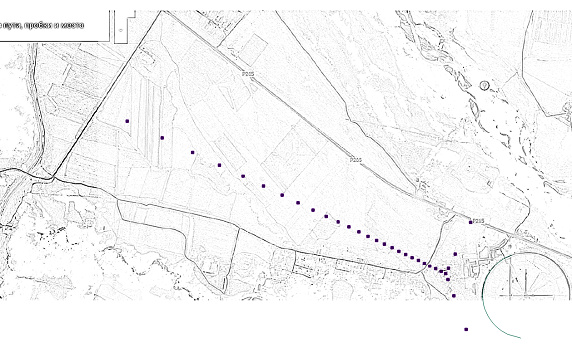
\includegraphics[width=1\linewidth]{./figures/RIF32-config1}} a) \\
\end{minipage}
\vfill
\begin{minipage}[h]{1\linewidth}
\center{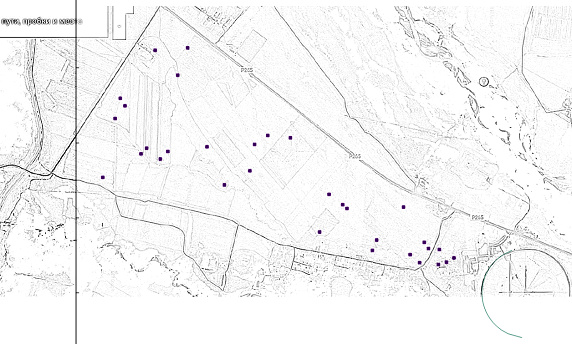
\includegraphics[width=1\linewidth]{./figures/RIF32-config2}} \\b)
\end{minipage}
\caption{Варианты расположения антенн РИФ--32: a) пример лучевого (регулярного) расположения антенн на территории, прилегающей к РАТАН-600, север справа, b) Пример случайного (нерегулярного) расположения антенн на территории, прилегающей к РАТАН-600, север справа.}
\label{fig:RIF32-config}
\end{figure}

\section{Научные задачи}

\subsection{Внегалактический нейтральный водород HI}
Наблюдения порядка миллиона галактик в линии нейтрального водорода на 70\% небесной сферы до красных смещений 0.3-0.4 дадут возможность лучше понять процессы формирования и эволюции галактик в ближней Вселенной.

Проведение глубокого обзора HI позволит провести прямые наблюдения HI в эмиссии на красных смещениях до z = 0.4 для большого числа галактик (порядка одного миллиона). Это даст возможность исследовать эволюцию барионной и тёмной материи, а также особенности звездообразования и образования галактик. 

Наблюдения распределения HI с высоким разрешением у нескольких сотен ближайших галактик, что позволит лучше понять внутреннюю динамику галактик, а также процессы звёздообразования. Эти данные могут быть скомбинированы с инфракрасными и UV наблюдениями, что даст возможность лучше понять эволюцию галактик и процессы в межзвёздной среде. Чувствительность таких наблюдений на предлагаемом инструменте будет лучше чем достигнутая в обзоре The HI Nearby Galaxy Survey (THINGS, VLA). Кроме того, эти наблюдения будут полезны в свете обзоров молекулярной и пылевой компоненты межзвёздной среды, которые проводились КА Hershel. 

\subsection{Наблюдения излучения в континууме}
Регистрация синхротронного излучения от более 50 млн галактик позволит уточнить детали эволюции и формирования галактик в течение длительного космологического времени, кроме того такие наблюдения помогут провести ключевые космологические тесты.

Большинство обзоров галактик (ATLAS, ELAIS, GOODS, COSMOS) проводились в оптическом и инфракрасном диапазонах, где велико поглощение за счёт пыли. Предлагаемый обзор в радиодиапазоне не только решит эту проблему, но и даст возможность получить информацию об активных ядрах галактик (AGN), недоступную в других диапазонах.

\subsection{Наблюдения в поляризации}
Наблюдения поляризованного излучения от более чем полумиллиона галактик даст возможность построить карты меры вращения (RM) с разрешением порядка 5 угл. минут, что в свою очередь позволит исследовать эволюцию магнитных полей в галактиках на протяжении длительного космологического времени.

\subsection{Изучение Галактики}
Инструмент даст возможность изучения эволюции межзвёздной среды в нашей Галактике, а также происходящих в ней химических и физических процессов.

\subsection{Эксперименты РСДБ}
Возможно объединение данного радиоинтерферометра с другими аналогичными инструментами в рамках системы Радиоинтерферометра со Сверхдлинными Базами для наблюдений интенсивных высокоэнергетических астрофизических явлений с высокми разрешением.

\subsection{Пульсары}
Проведение специальных обзоров позволит обнаружить и измерить порядка 1000 новых радиопульсаров. Поисковые наблюдения на частотах больше 10 ГГц позволят обнаружить несколько сотен новых радиопульсаров, некоторые из которых обращаются вокруг сверхмассивной чёрной дыры в центре Галактики. Результаты этих наблюдений могут быть интегрированы с международную программу по регистрации низкочастотных гравитационных волн.

\subsection{Транзиентные и быстропеременные явления}
Инструмент даст возможность обнаружения изучения в радиодиапазоне быстропеременных и транзиентных явлений, таких как гамма-всплески, сверхновые, быстрые радио всплески (FRB) и быстропеременные радиоисточники.

\section{Моделирование}

\section{Заключение}

\section*{Благодарности}

\begin{thebibliography}{1}
\bibitem{Hagen} Jon B. Hagen, {\em Radio-frequency electronics. Circuits and application}, Second ed., Cambridge University Press, Cambridge, 2009 %, p.380.

\end{thebibliography}

\end{document}